\chapter{Artificial Neural Networks}

\section{Background and basic ideas}

This section will provide a very basic introduction to the
field of Artificial Neural Networks (ANN or NN) - the technology
with many decades of history and actively growing in last 10-15 years.
The advances in high-performance computing and easy access
to a variety of datasets made NN one of central technologies
in machine learning and artificial intelligence.

As the name suggests NN are somehow related to the structure of a brain.
The history and relationships between developments in AI and in
neuroscience are not subjects of this course but we'll see that NN
structure and operations resemble two elements of biological
neural systems:

\begin{enumerate}
\item threshold-like activation potential -- for a neuron to "fire"
the electrical potential must exceed some level.
\item neurons are interconnected -- they form a complex network.
\end{enumerate}

The ideas on NN in artificial intelligence only partially came from
biology\footnote{The biological principles are usually seen in AI as
metaphors rather than theoretical foundation.}. The main area
where NN principles are rooted is the question of computability --
the fundamental problem in computer science. Names of Turing,
von Neumann, Kolmogorv are among many others who structured the field.

Let's now formulate a basic problem. We have an input -- numerical value,
a list of numerical values, image (can be presented as a list of numbers),
etc. -- and an associated output. For example the input can be an image
and the output a boolean value indicating that the image represents a cat.
We want to build a model $F$ that can associate output to a given input.
Fore the example above -- to find all images with cats.

In other words, for input a set of inputs $X$ we want to find
function $F$ that maps $X$ into a set of outputs $Y$:
$$
F: X \rightarrow Y
$$
Or for multi-dimensional $X$ (${x_i}, i=1..N$) and $Y$ (${y_i}, i=1..M$):

\bigskip
\begin{center}
\begin{tikzpicture}[node distance = 4mm]
\node (adc) [draw,minimum size=16mm] {F};
%
\coordinate[above left = of adc.west]   (a1);
\coordinate[below = of a1]              (a2);
\coordinate[below = of a2]              (a3);
\coordinate[above right= of adc.east]   (b1);
\coordinate[below = of b1]              (b2);
\coordinate[below = of b2]              (b3);
%
\foreach \i [count=\xi from 1] in {$x_1$, $x_2$, $\dots$}
    \draw[-latex'] (a\xi) node[left] {\i} -- (a\xi-| adc.west);
\foreach \i [count=\xi from 1] in {$y_1$, $y_2$, $\dots$}
    \draw[-latex'] (adc.east |- b\xi) -- (b\xi) node[right] {\i};
\end{tikzpicture}
\end{center}

In this section we'll consider only one type of NN -- multi-layer
perceptron, the generalization of single-layer perceptron. Let's
start with the latter and first assume that there is only one output
value (the doesn't affect the discussion as we can assume that we have
an individual function $F$ for each output component):

\bigskip
\begin{center}
\begin{tikzpicture}[node distance = 4mm]
\node (adc) [draw,minimum size=16mm] {F};
%
\coordinate[above left = of adc.west]   (a1);
\coordinate[below = of a1]              (a2);
\coordinate[below = of a2]              (a3);
\coordinate[above right= of adc.east]   (b1);
%
\foreach \i [count=\xi from 1] in {$x_1$, $x_2$, $\dots$}
    \draw[-latex'] (a\xi) node[left] {\i} -- (a\xi-| adc.west);
\foreach \i [count=\xi from 1] in {$y$}
    \draw[-latex'] (adc.east |- b\xi) -- (b\xi) node[right] {\i};
\end{tikzpicture}
\end{center}


\subsection{Single-layer perceptron}

The single-layer perceptron scheme is:
$$
\begin{matrix}
x_1 \rightarrow w_1\cdot x_1 & \\
x_2 \rightarrow w_2\cdot x_2 & \\
\dots &
\rightarrow \sum_{i=1}^N w_i\cdot x_i + w_0 \rightarrow f(\sum_{i=1}^N w_i\cdot x_i + w_0) \rightarrow y \\
x_i \rightarrow w_i\cdot x_i & \\
\dots & 
\end{matrix}
$$
We first calculate a weighted sum of input components
and then calculate function $f(\cdot)$ of the sum.
The choice of $f$ is crucial. It's easy to see that the linear function
$f(x) = a\cdot x + b$ is the equivalent of linear dependence
between $X$ and $Y$:
$$
f(\sum_{i=1}^N w_i\cdot x_i + w_0) =
a\cdot\sum_{i=1}^N w_i\cdot x_i + a\cdot w_0 + b =
\sum_{i=1}^N w'_i\cdot x_i + w'_0
$$
where $w'_i = a\cdot w_i$ and $w'_0 = a*w_0+b$.

The common choice is a smoothed version of a step function
(sigmoid). The step function:
$$
f(x) = \left\{ 
\begin{array}{ll}
0 & x < 0 \\
1 & x \geq 0
\end{array}
\right.
$$

\begin{center}
\begin{tikzpicture}
\draw[->] (-2.2,0) -- (2.2,0) node[right] {$x$};
\draw[->] (0,-0.5) -- (0,1.5) node[above] {$y$};
\draw[domain=-2:0,smooth,ultra thick,variable=\x] plot ({\x},{0});
\draw[domain=0:2,smooth,ultra thick,variable=\x] plot ({\x},{1});
\end{tikzpicture}
\end{center}

Sigmoid:
$$
f(x) = \frac{1}{1+\exp(-x)}
$$
\begin{center}
\begin{tikzpicture}
\draw[->] (-3.2,0) -- (3.2,0) node[right] {$x$};
\draw[->] (0,-0.5) -- (0,1.5) node[above] {$y$};
%\draw[scale=0.5,domain=-3:3,smooth,variable=\x,blue] plot ({\x},{\x*\x});
\draw[domain=-2:2,smooth,ultra thick,variable=\x] plot ({\x},{1/(1+exp(-4*\x))});
\end{tikzpicture}
\end{center}
Sigmoid is close to the step function for big positive and negative values 
of $x$, and smooth behaviour at $x=0$ makes it convenient for a number
of applications.

One of the other options is RELU (REctified Linear Unit):

$$
f(x) = \left\{ 
\begin{array}{ll}
0 & x < 0 \\
x & x \geq 0
\end{array}
\right.
$$
\begin{center}
\begin{tikzpicture}
\draw[->] (-2.2,0) -- (2.2,0) node[right] {$x$};
\draw[->] (0,-0.5) -- (0,2.2) node[above] {$y$};
\draw[domain=-2:0,smooth,ultra thick,variable=\x] plot ({\x},{0});
\draw[domain=0:2,smooth,ultra thick,variable=\x] plot ({\x},{\x});
\end{tikzpicture}
\end{center}

This is not the complete list of functions used in NN,
there exist functions with more complex and not always deterministic
behaviour, but the idea remains the same -- some non-linear and
often threshold-like function.

Let's see how this works for simple dependencies between $X$ and $Y$.
For the exercise we'll choose step function:
and basic logical operations (NOT, AND, OR, XOR) as they are
simple enough to implement without coding and get an idea of the
approach.

\textbf{Logical NOT}.
Here is the table of possible cases\footnote{It's common to use 0
to denote False and 1 to denote True}:
\begin{center}
\begin{tabular}{c|c}
X & NOT X \\
\hline
1&0\\
0&1
\end{tabular}
\end{center}
Consider the following weights:
$$
w_0 = 0.5,\ \ w_1 = -1
$$
$$
Y = f(-X+0.5)
$$
\begin{center}
\begin{tabular}{c|c}
X & Y \\
\hline
1&$f(-1\cdot 1+0.5)=f(-0.5)=0$ \\
0&$f(-1\cdot 0+0.5)=f(0.5)=1$ 
\end{tabular}
\end{center}
As we can see $Y$ corresponds to $NOT X$

\textbf{Logical AND}. The same steps:
\begin{center}
\begin{tabular}{c|c|c}
$X_1$ & $X_2$ & $X_1 AND X_2$ \\
\hline
0&0&0 \\
0&1&0 \\
1&0&0 \\
1&1&1
\end{tabular}
\end{center}
$$
w_0 = -1, \ \ w_1 = 0.5, \ \ w_2 = 0.5
$$
$$
Y = f(-1+0.5*X_1+0.5*X_2)
$$
\begin{center}
\begin{tabular}{c|c|c}
$X_1$ & $X_2$ & $Y$ \\
\hline
0&0&$f(-1+0.5\cdot 0+0.5\cdot 0) = f(-1) = 0$   \\
0&1&$f(-1+0.5\cdot 0+0.5\cdot 1) = f(-0.5) = 0$ \\
1&0&$f(-1+0.5\cdot 1+0.5\cdot 0) = f(-0.5) = 0$ \\
1&1&$f(-1+0.5\cdot 1+0.5\cdot 1) = f(0) = 1$
\end{tabular}
\end{center}

\textbf{Logical OR}. The same steps:
\begin{center}
\begin{tabular}{c|c|c}
$X_1$ & $X_2$ & $X_1 OR X_2$ \\
\hline
0&0&0 \\
0&1&1 \\
1&0&1 \\
1&1&1
\end{tabular}
\end{center}
\begin{tcolorbox}
\textbf{Assignment:} this case is similar to AND, find $W_0, \ W_1, \ W_2$.
\end{tcolorbox}

\textbf{Logical XOR (exclusive OR)}
\begin{center}
\begin{tabular}{c|c|c}
$X_1$ & $X_2$ & $X_1 XOR X_2$ \\
\hline
0&0&0 \\
0&1&1 \\
1&0&1 \\
1&1&0 \\
\end{tabular}
\end{center}

Here we have a problem: single-layer perceptron cannot compute
XOR for all four combinations of arguments.
Let's see what's different between XOR and other two variable
functions (AND, OR).To do this we'll 
represent functions in the following way:

\begin{center}
AND

\medskip
\begin{tabular}{c|c}
0&0 \\
\hline
0&1
\end{tabular}
\end{center}

\medskip
\begin{center}
OR

\medskip
\begin{tabular}{c|c}
0&1 \\
\hline
1&1
\end{tabular}
\end{center}

\medskip
\begin{center}
XOR

\medskip
\begin{tabular}{c|c}
0&1 \\
\hline
1&0
\end{tabular}
\end{center}

We can find that zeros and ones in AND and OR form "islands"
that can be separated by a single line -- just apply a ruler
and find that you can have all zeros in AND above the ruler
and one below the ruler. The same can be done for OR:

\bigskip
\begin{center}
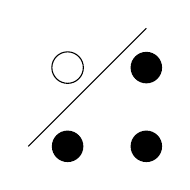
\begin{tikzpicture}
\draw (-0.5,0) -- (1,1.5);
\draw (0,1) circle (0.2);
\fill[black] (0,0) circle (0.2);
\fill[black] (1,0) circle (0.2);
\fill[black] (1,1) circle (0.2);
\end{tikzpicture}
\end{center}
\bigskip



XOR is different -- you need at least two lines to separates
zeros and ones:

\bigskip
\begin{center}
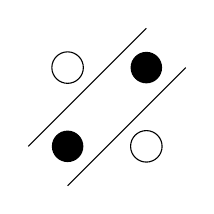
\begin{tikzpicture}
\draw (-0.5,0) -- (1,1.5);
\draw (0,-0.5) -- (1.5,1);
\draw (0,1) circle (0.2);
\fill[black] (0,0) circle (0.2);
\draw (1,0) circle (0.2);
\fill[black] (1,1) circle (0.2);
\end{tikzpicture}
\end{center}

 The linear separability is an important feature.
It can be introduced in a formal way and it's possible to
prove that a single layer perceptron cannot implement non-linear-separable
function.

\subsection{Multi-layer perceptron}
Perceptron structure can include a hidden layer or layers. 

\begin{tikzpicture}[
plain/.style={draw=none,fill=none,},
net/.style={matrix of nodes, nodes={draw,circle,inner sep=8.5pt},
    nodes in empty cells,column sep=0.6cm,row sep=-11pt},
>=latex]

\matrix[net] (mat)
{
|[plain]| \parbox{1cm}{\centering Input\\layer} & |[plain]| \parbox{1cm}{\centering Hidden\\layer} & |[plain]| \parbox{1cm}{\centering Output\\layer} \\
    |[plain]| & \\
    & |[plain]| \\
    |[plain]| & &  \\
    & |[plain]| \\
    |[plain]| & &  \\
    & |[plain]| \\
    |[plain]| & \\
};
\foreach \ai [count=\mi ]in {3,5,7}
\draw[<-] (mat-\ai-1) -- node[above] {$x_{\mi}$} +(-2cm,0);
\foreach \ai in {3,5,7}
{\foreach \aii in {2,4,...,8}
    \draw[->] (mat-\ai-1) -- (mat-\aii-2);
}
\foreach \ai in {2,4,...,8}
\draw[->] (mat-\ai-2) -- (mat-6-3);

\foreach \ai in {2,4,...,8}
\draw[->] (mat-\ai-2) -- (mat-4-3);

\foreach \ai [count=\mi ]in {4,6}
\draw[->] (mat-\ai-3) -- node[above] {$y_{\mi}$} +(2cm,0);
\foreach \ai in {3,5,7}
{\foreach \aii in {2,4,...,8}
    \draw[->] (mat-\ai-1) -- (mat-\aii-2);
}
\end{tikzpicture}



Calculations of output values include two steps:
first we calculate outputs of hidden layer nodes and then use
them to calculate output. The output $z_k$ of $k$-th node of the
hidden layer ($k=1..N_h$):
$$
z_k = f( \sum_{i=1}^N w_{ik}^1\cdot x_i + w_{0k}^1 )
$$
where $w_{ik}^1$ is the weight of connection between $i$-th
input node and $k$-th hidden layer node. Output values $y_j$ are:
$$
y_j = f( \sum_{i=1}^{N_h} w_{kj}^2\cdot z_k + w_{0j}^2 )
$$
Note that the upper index 2 in $w_{kj}^2$ doesn't indicate
square of the number, it refers to the second set of weights --
weights between hidden layer nodes and output nodes.

We can create NN with more than one hidden layer, but the 
idea remains the same: we want to build a layered structure
Where the output of a node is a function of a weighted sum of
of outputs of the previous layer nodes. Those weights have to be
calculated in the process known as "learning": given the set of
input/output values we want to choose weights so that the total
error of calculated outputs is minimal. For example, if we have
1000 images and 500 of them are with cats we want to train NN
that can correctly identify the most of those 500 images
\footnote{At this moment we do not consider the question of
using NN in- and out-of-sample.}.

To do this we can introduce a formal measure of the error that
depends on the set of input/output values $X$ and $Y$ and
all weights $W$ ($w^{k}_{ij}$):
$$
ERR(X,Y,W)
$$
The learning is the procedure of finding weights $W$ that minimize
the error:
$$
ERR(X,Y,W) \rightarrow\min_{W}
$$

The common approach to NN training is called back propagation.
The idea and implementation of the approach is out of the scope of
this course as they require understanding of basic optimization
techniques. Instead we'll be using programming libraries where
all required functionality is available without going deep into
the theory.

We'll consider multi-layer perceptron only -- the course
doesn't cover important and interesting cases of Convolutional NN (CNN),
Recurrent NN (RNN), Long-Short Term Memory (LSTM),
Hopfield networks (RNN with binary node states), and others.
Model-specific modifications do not change the idea of the learning
 -- we want to choose weights and sometimes
other parameters to minimize the output approximation error.

\section{Neural networks and rules of "Life"}

In the previous sections we were analysing systems with known
behaviour -- mazes, 8-pazzle, Tic-Tac-Toe game. Now let's try to identify
rules from observations: we'll be looking at some system and trying
to replicate it's behaviour without knowing underlying rules.

As
"Life" - the game introduced by Conway
has simple rules, resulting in interesting behaviour. "Life"
is an example of cellular automata -- the system that consists
of cells on a rectangular grid with behaviour of a cell defined
by its neighbors:

\bigskip
\begin{center}
\begin{tabular}{c|c|c|c|c}
 & & & & \\
\hline
 & $\cdot$ & $\cdot$ & $\cdot$ & \\
\hline
 & $\cdot$ & \cellcolor{black} & $\cdot$  & \\
\hline
 & $\cdot$ & $\cdot$ & $\cdot$ & \\
\hline
 & & & & 
\end{tabular}
\end{center}
\bigskip

Each cell can be alive or dead. A cell changes the
state depending on the own state and the state of 8 neighbors:
Rules of the state change:

\begin{enumerate}
\item A live cell remains a live cell if it has 2 or 3 live neighbors, otherwise
it dies.
\item A dead cell becomes a live cell if it has 3 live neighbors,
otherwise it remains dead.
\end{enumerate}

Here are several examples of the static structures - they do not
change:

\textbf{Block} -- each live cell has three live neighbors, each dead cell
has not more than two live cells:
\begin{center}
\begin{tabular}{c|c|c|c}
 & & & \\
\hline
 & \cellcolor{black} & \cellcolor{black} & \\
\hline
 & \cellcolor{black} & \cellcolor{black} & \\
\hline
 & & &  
\end{tabular}
\end{center}
\bigskip

\textbf{Boat} (confirm that this configuration is a static one):
\begin{center}
\begin{tabular}{c|c|c|c|c}
 & & & & \\
\hline
 & \cellcolor{black} & \cellcolor{black} & & \\
\hline
 & \cellcolor{black} & & \cellcolor{black} & \\
\hline
 & & \cellcolor{black} & & \\
\hline
 & & & & 
\end{tabular}
\end{center}
\bigskip

Configurations with periodic behaviour:

\textbf{Blinker}
\begin{center} %%% blinker - begin

\begin{tabular}{cccccc}

\begin{tabular}{c|c|c|c|c}
 & & & & \\
\hline
 & & \cellcolor{black} & & \\
\hline
 & & \cellcolor{black} & & \\
\hline
 & & \cellcolor{black} & & \\
\hline
 & & & & 
\end{tabular}

&
$\rightarrow$
&

\begin{tabular}{c|c|c|c|c}
 & & & & \\
\hline
 & & & & \\
\hline
 & \cellcolor{black} & \cellcolor{black} & \cellcolor{black} & \\
\hline
 & & & & \\
\hline
 & & & & 
\end{tabular}

&
$\rightarrow$
&

\begin{tabular}{c|c|c|c|c}
 & & & & \\
\hline
 & & \cellcolor{black} & & \\
\hline
 & & \cellcolor{black} & & \\
\hline
 & & \cellcolor{black} & & \\
\hline
 & & & & 
\end{tabular}

&
$\rightarrow\dots$
\end{tabular}
\end{center} %%% blinker - end
\bigskip

\textbf{Toad} 
\begin{center} %% Toad -- begin
\begin{tabular}{cccc}

\begin{tabular}{c|c|c|c|c|c}
 & & & & &\\
\hline
 & & & \cellcolor{black} & & \\
\hline
 & \cellcolor{black} & & & \cellcolor{black} & \\
\hline
 & \cellcolor{black} & & & \cellcolor{black} & \\
\hline
 & & \cellcolor{black} & & & \\
\hline
 & & & & &
\end{tabular}

&
$\rightarrow$
&

\begin{tabular}{c|c|c|c|c|c}
 & & & & &\\
\hline
 & & & & & \\
\hline
 & & \cellcolor{black} & \cellcolor{black} & \cellcolor{black} & \\
\hline
 & \cellcolor{black} & \cellcolor{black} & \cellcolor{black} & & \\
\hline
 & & & & & \\
\hline
 & & & & &
\end{tabular}
&
$\rightarrow\dots$

\end{tabular}
\end{center} %% Toad -- end

\begin{tcolorbox}
\textbf{Assignments:}
\begin{enumerate}
\item Use paper to draw changes in the states for the glider:
\begin{center}
\begin{tabular}{c|c|c|c|c}
 & & & & \\
\hline
 & & \cellcolor{black} & & \\
\hline
 & & & \cellcolor{black} & \\
\hline
 & \cellcolor{black} & \cellcolor{black} & \cellcolor{black} & \\
\hline
 & & & & 
\end{tabular}
\end{center}
\item Write Python function that returns new state for the central cell
on a 3x3 grid.
\item Write Python function that returns new state for an cell
given by coordinates (i,j) on a board:

\begin{center}
\begin{tabular}{c|c|c|c|c}
 & & & & \\
\hline
 & (i-1,j-1) & (i-1,j) & (i-1,j+1) & \\
\hline
 & (i,j-1) & \textbf{(i,j}) & (i,j+1) & \\
\hline
 & (i+1,j-1) & (i+1,j) & (i+1,j+1) & \\
\hline
 & & & & 
\end{tabular}
\end{center}

\end{enumerate}
\end{tcolorbox}

A cell on a boundary has only 5 neighbors
which may make it die faster than cells inside:

\begin{center}
\begin{tabular}{c|c|c|c|c}
 & & & & \\
\hline
 & & & & \\
\hline
 & $\cdot$ & $\cdot$ & $\cdot$ & \\
\hline
 & $\cdot$ & \cellcolor{black} & $\cdot$ & \\
\hline
\end{tabular}
\end{center}

To avoid this we can
introduce periodic conditions: we'll assume that neighbors of a cell
on a border include also three cells on the opposite border:

\begin{center}
\begin{tabular}{c|c|c|c|c}
\hline
 & $\cdot$ & $\cdot$ & $\cdot$ & \\
\hline
 & & & & \\
 & & & & \\
\hline
 & $\cdot$ & $\cdot$ & $\cdot$ & \\
\hline
 & $\cdot$ & \cellcolor{black} & $\cdot$ & \\
\hline
\end{tabular}
\end{center}

In this case the following starting configuration doesn't disappear
(live cells have only one live neighbor without taking into account
cells on the opposite border), but becomes an equivalent to the "Block"
(see above).

\begin{center}
\begin{tabular}{c|c|c|c|c|c}
\hline
 & & \cellcolor{black} & \cellcolor{black} & & \\
\hline
 & & & & & \\
\hline
 & & & & & \\
\hline
 & & & & & \\
\hline
 & & \cellcolor{black} & \cellcolor{black} & & \\ 
\hline
\end{tabular}
\end{center}

The same conditions can be applied to left and right borders.

\begin{tcolorbox}
\textbf{Assignments:}
\begin{enumerate}
\item Write Python function that returns new state for an cell
given by coordinates (i,j) on a board with periodic conditions.
\item Write Python function that updates a board of an arbitrary
size. Assume periodic conditions and add function that prints
a board (use space symbol for a dead cell and asterisk for a live cell).
\end{enumerate}
\end{tcolorbox}












\begin{tcolorbox}
\textbf{Python:} learn about \textbf{scikit-learn} library.
\end{tcolorbox}




